\documentclass[
  a4paper,BCOR10mm,oneside,
  bibtotoc,idxtotoc,
  headsepline,footsepline,% also activate headinclude and footinclude
  fleqn,openbib
]{scrbook}
\usepackage[automark]{scrpage2}
\usepackage[ngerman,english]{babel}% default language as last entry
\usepackage[utf8]{inputenc}
\usepackage{amsmath} 
\usepackage{amsfonts}
\usepackage{amssymb}
\usepackage{graphicx}
\usepackage{lastpage}% to get last page use \pageref{LastPage}
\usepackage[refpage,intoc]{nomencl}% for nomenlature Abkuerzungsverzeichnis
\usepackage{listings}
\usepackage{color}
\usepackage{hyperref}
\usepackage{bm}
\usepackage{cleveref}
\usepackage{caption,setspace}
\usepackage{verbatim}
\definecolor{mygreen}{rgb}{0,0.6,0}
\definecolor{mygray}{rgb}{0.5,0.5,0.5}
\definecolor{mymauve}{rgb}{0.58,0,0.82}

\lstset{ %
  backgroundcolor=\color{white},   % choose the background color; you must add \usepackage{color} or \usepackage{xcolor}
  basicstyle=\footnotesize,        % the size of the fonts that are used for the code
  breakatwhitespace=false,         % sets if automatic breaks should only happen at whitespace
  breaklines=true,                 % sets automatic line breaking
  captionpos=b,                    % sets the caption-position to bottom
  commentstyle=\color{mygreen},    % comment style
  deletekeywords={...},            % if you want to delete keywords from the given language
  escapeinside={\%*}{*)},          % if you want to add LaTeX within your code
  extendedchars=true,              % lets you use non-ASCII characters; for 8-bits encodings only, does not work with UTF-8
  frame=single,	                   % adds a frame around the code
  keepspaces=true,                 % keeps spaces in text, useful for keeping indentation of code (possibly needs columns=flexible)
  keywordstyle=\color{blue},       % keyword style
  language=Octave,                 % the language of the code
  otherkeywords={*,...},           % if you want to add more keywords to the set
  numbers=left,                    % where to put the line-numbers; possible values are (none, left, right)
  numbersep=5pt,                   % how far the line-numbers are from the code
  numberstyle=\tiny\color{mygray}, % the style that is used for the line-numbers
  rulecolor=\color{black},         % if not set, the frame-color may be changed on line-breaks within not-black text (e.g. comments (green here))
  showspaces=false,                % show spaces everywhere adding particular underscores; it overrides 'showstringspaces'
  showstringspaces=false,          % underline spaces within strings only
  showtabs=false,                  % show tabs within strings adding particular underscores
  stepnumber=2,                    % the step between two line-numbers. If it's 1, each line will be numbered
  stringstyle=\color{mymauve},     % string literal style
  tabsize=2,	                   % sets default tabsize to 2 spaces
  title=\lstname                   % show the filename of files included with \lstinputlisting; also try caption instead of title
\makenomenclature
}

% define header and footer
\pagestyle{scrheadings}
\clearscrheadfoot % clear header and footer
\automark[section]{chapter}% !!! Wouldn't do that at oneside documents!!!
\ihead[]{\leftmark}% header left part
\ohead[]{\rightmark}% header right part
%\ifoot{Name}% footer left part
%\cfoot{Thema}% footer middle part
\makeatletter
% use different foot at front and main matter
\g@addto@macro{\mainmatter}{%
  \ofoot[{\usekomafont{pagenumber}Page \pagemark\ of \pageref{LastPage}}]
    {\usekomafont{pagenumber}Page \pagemark\ of 
      \pageref{LastPage}}% footer right part
}
\g@addto@macro{\frontmatter}{%
  \ofoot[\pagemark]{\pagemark}%
}
\makeatother


\begin{document}
\frontmatter% title pages are not numbered but counted!
\begin{titlepage}
  \raggedright% Use a different title style
  \null% page started
  \thispagestyle{empty}
  \selectlanguage{english}
  \vspace{4\baselineskip}
  \begin{tabular}{|ll@{}}
    & \\[\baselineskip]
    & \large Midtherm Report\\
    & \large Jan Grzegorzewski \\[\baselineskip]
    & \huge\textbf{Reaction-diffusion dynamics} \\
    & \huge\textbf{with fractional Brownian motion}\\[\baselineskip]
    & \large Summer term: 2016\\[2\baselineskip]
  \end{tabular}
\end{titlepage}

\tableofcontents
\listoffigures
%\listoftables

\mainmatter
\selectlanguage{ngerman}
\selectlanguage{english}
\printnomenclature
\clearpage

\newtheorem{mydef}{Definition}
\newcommand{\norm}[1]{\left\lVert#1\right\rVert}

\chapter{Motivation}
Anomalous diffusion can be observed in many different areas of nature in particular related to heterogeneous media like porous rocks, random resistor networks and crowded biological media with its prominent phenomena macro molecular crowding, confinement and macromolecular adsorption \cite{Minton2006}. These environments exhibit remarkable characteristics like anomalous diffusion with its most popular power-law behaviour of the Mean-Square-Displacement ($MSD\propto t^{\alpha}$) \cite{Hofling2013}, which is violating the Einstein formula $MSD=2 d D t$ and thereby the central limit theorem. Various theoretical models try to encounter the power-law behaviour of the MSD. These models have the main phenomenon, thus the power-law behaviour of the Mean-Square-Displacement in common, but differ in some other observables, due to different origins of the anomalous power-law behaviour.One of these models which account this phenomenon is fractional Brownian motion (fBm). It was first introduced as family of Gaussian random function by Mandelbrot and Van Ness in 1968 and motivated by examples in economics \cite{Mandelbrot1968}. In contrast to different models of anomalous diffusion fBm nature is plainly phenomenological in respect to the power-law behaviour of the MSD and thus perfectly qualifies as a starting point to study effects resulting from a power-law  MSD. \newline 
This thesis is going to focus on fBm especially in respect to Reaction and Diffusion Dynamics.  Fick’s law is violated for diffusion in disordered media \cite{Havlin1987}, which is essential in the derivation of the famous equation of the rate for diffusion-controlled reaction processes $k=4 \pi D R_0$. Thus it is failing miserably in describing Reaction and Diffusion Dynamics while anomalous motion is present. The aim of the work is to bring diffusion-controlled reactions and fBm together for this purpose a fBm integrator will be implemented into a particle-based Reaction  Diffusion Dynamics software which is acting on a macromolecular level. It is coarse-graining molecules into spherical particles. Usually using Brownian or Lagevin motion as the integrator. A Fractional Brownian Motion Integrator may be an elegant way of adding an approximation due to a crowded environment. The phenomenon of anomalous motion can also be studied with conventional integrators by actually building a crowded environment e.g. by adding obstacles. Nevertheless, the fBm approach could save computational time since it is not necessary to simulated each particle  explicitly which builds up the crowded environment. Furthermore different studies show that heterogeneous environments have influences on particle segregation in the presents of reactions \cite{Berry2002}, which is an interesting phenomena of self-organization.\newline
Having an Introduction set, chapter 2 deals with the theoretical foundation for fBm. Subsequently, due to computational reasons these theoretical elaborations need to be transferred into discrete space and finally casted into an algorithm. In the following some properties of the algorithm are studied. In Chapter 3, the theoretical foundation for reactions are going to be set. The final chapter 4 gives an outlook of the master thesis.  

\chapter{Theory}
\section{Brownian Motion}
Fractional Brownian motion is a more general family of Gaussian random function than standard Brownian motion. The following section will explore in more detail the theoretical foundation for Brownian motion and normal diffusion. After acquiring the required knowledge also the more general case of fBm will be studied. \newline
Standard Brownian Motion is a very important and good studied stochastic process. It describes the erratic motion for mesoscopic particles, which  first have been documented by Jan Ingenhousz in 1785, in particular for coal dust on the surface of alcohol\cite{Hofling2013}. Later on in 1827 Robert Brown observed the erratic motion of pollen grains.  Brownian Motion has an Gaussian propagator which has its origin in the Central Limit Theorem (CLT) for a sum of of independent random variables. Lets assume a set of $N$ independent variables $\{X_i\}$ with a finite variance $ \sigma_i^2=\langle X_{i}^2\rangle $ and the mean $\langle X_{i}\rangle = 0$. The definition of a another random variable $Y$ is given by:
 \begin{align}
  Y = \frac{1}{\sqrt{N}} \sum_{j=1}^N X_j \label{eq:CLT}
 \end{align}
This scenario in which a random variable is defined of the sum of another can be observed generically in nature. The seemingly innocent assumption of independence for the random variable $\{X_i\}$ in the summation results in the limit of large N $\rho(y)dy=P(y<Y<y+dy)$ in an Gaussian distribution $\rho(y)$  .
\begin{align}
 \rho(y) =\frac{1}{\sqrt{2 \pi} \sigma } e^{-\frac{y^2}{2 \sigma^2}}
\end{align}
A calculation of this very interesting result can be found in the Appendix \ref{append:CLT}.    Microscopic processes, which result in independent random position changes of an particle and add up over time, thus have a Gaussian distribution function for the overall change in position. With  Bayes' theorem and an initial delta-distribution one can show that transition probability $T_{t}(y|0) = \rho_{t}(y)$ is equivalent to the particle density function. One can find the calculation in the Appendix \ref{baystheorem}. The above-mentioned elaborations motivate the reason for a process with a Gaussian transition probability, which is standard Brownian motion.
\begin{mydef}
Standard Brownian motion is a stochastic process $ \{ W_t \}_{t\geq0}: \Omega \rightarrow \mathbb{R}^d$ with $ W_t(\omega)$ being the position of a particle with $\omega \in \Omega$ at time $t \in T$ in the observation time $T =[0, \infty)$. It has a fixed $x \in \mathbb{R}^d$ as its origin. The transition probabilities are \cite{LectureFelix}: 
\begin{align}
T_{t}(y|x) & := (2 \pi t)^{- \frac{d}{2}} e^{- \frac{||x-y||^2}{2 t}} \text{for } y \in \mathbb{R}^d, t>0 \\ \nonumber
T_{0}(y|x) & = \delta(x-y) 
\end{align}
\end{mydef}
In the following some properties of Brownian motion are discussed:\\
\begin{itemize} \label{bscaling}
\item Brownian motion is a Gaussian process with mean $E^x[W_t]=x$, $W_o=x$.
Since $ E^x[(W_{t_i}-W_{t_{i-1}})(W_{t_j}-W_{t_{j-1}})]=0 $  all its increments $\{W_{t_1},W_{t_2}-W_{t_1},...,W_{t_k}-W_{k-1}\}$ are independent.

\item Brownian motion has stationary increments since ${W_{t-h}-W_{h}}$ has the same distribution for all $h>0$.

\item  Brownian scaling $\{\hat{W}_t := \frac{1}{c} W_{c^2 t} \}_{t\geq0}$ if $\{W_t\}_{t \geq 0}$  is also a Brownian motion. Therefore Brownian motion has self-similar and fractal paths. 
\end{itemize}
Introducing Fick's second law of diffusion, which predicts how diffusion causes the concentration to change over time:
\begin{align}
 \frac{\partial}{\partial t} c(\bm{r},t) = - \nabla J (\bm{r},t) = D  \Delta c(\bm{r},t) \qquad \text{ with } \qquad \Delta= \nabla^2  \label{eq:ficks}
\end{align}
With Fick's first law $-J(\bm{r},t)=\nabla c(\bm{r},t)$ and $D$ being the flux of particles and the diffusion coefficient, respectively. Fick's first law is a result from the linear response theory. Fick's second law can be derived from the continuity equation and Fick's first law. The Concentration $c(\bm{r},t)$ can be interpreted as a probability distribution, if properly normalized  $\int d\bm{r} c(\bm{r},t)=1$. For further calculation the mathematical description of a transition probability of Brownian motion will be replaced with a more physical description of a propagator:
\begin{align}
 P(\bm{r},t)=  \left(\frac{2 \pi \delta \bm{r}^2(t)}{d}\right)^{- \frac{d}{2}} e^{- \frac{\bm{r}^2 d}{2 \delta \bm{r}^2(t)}} \label{propagator}
\end{align}
One can show that the propagator is solving \cref{eq:ficks} for $\delta \bm{r}^2(t)=2dDt$ for the meaningful initial condition of vanishing concentration at boundaries: 
\begin{align}
c(\pm \infty,t)=0
\end{align}
The calculation can be found in the Appendix \ref{einsteinrealtionappendix}.
For further references a scale free form of the Gaussian propagator will be introduced. It is a more intuitive consequent of Brownian scaling.
\begin{align}
P(\bm{r},t)= r^{-d} \mathcal{P}_{gauss}(\hat{\bm{r}})  \qquad \text{with} \qquad \hat{\bm{r}} = \frac{\bm{r}}{\sqrt{2Dt}}
\end{align}



\section{Fractional Brownian Motion}
(at some point start comparing to the section properties of brownian motion)
In this section the theoretical foundation for Fractional Brownian Motion will be set and related to standard Brownian Motion. \\
In the previous section the MSD has been shown to be linear with time as a result of the central limit theorem. In normal liquids this behaviour can be be seen already at time scales higher than picosecends \cite{Hofling2013}. Nevertheless many experiments show that the MSD has a power law behaviour ( $\delta r ^2 (t) \propto t^{\alpha}$ for  $0 < \alpha < 1$ ). Thus the central limit theorem does not hold, not even for long time scales. It can be shown that persistent correlations of the increments are present. In soft matter, like polymers, subdiffusive behaviour is typically present in an time window but finally the linear MSD takes over. Fractional Brownian Motion instead examines the case that the central limit theorem is violated for all time scales. The basic feature of fBm's is that the "span of interdependence" between their increments can be said to be infinite\cite{Mandelbrot1968}\\
\begin{mydef}
Just like standard Brownian motion, fBm is a Gaussian process $\{X_t\}_{t\geq0}: \Omega \rightarrow \mathbb{R}^d$. Therefore it is fully specified by its mean $E[X_t]=0$ and its (co)variance function $Cov[X_t,X_s]\stackrel{stationary} {=}C(t-s)=E[\delta X_{t-s}^* X_{0}]$ . As standard Brownian motion it has a Gaussian propagator \ref{propagator}: 
\begin{align*}
P(\bm{r},t)&=  \left(\frac{2 \pi \delta \bm{r}^2(t)}{d}\right)^{- \frac{d}{2}} e^{- \frac{\bm{r}^2 d}{2 \delta \bm{r}^2(t)}} 
\end{align*}
but in contrast to Brownian motion its variance is different:
\begin{align*}
\delta r^{2}(t)= < \Delta R(t)>=2dK_{\alpha}t^{\alpha}
\end{align*}
with $K_{\alpha}>0$  being the generalized diffusion coefficient.
\end{mydef}
In the following some statistical tools are defined. They are important as the increments of fBm are no longer assumed to be independent. 
\begin{itemize}
 \item The single particle density $\rho(\bm{r},t)=\delta(\bm{r}-\bm{R}(t))$ describes the density of a particle which is localized at position $\bm{R}(t)$. Its correlation function $P(\bm{r}-\bm{r}',t-t')= V\langle\rho(\bm{r},t) \rho(\bm{r}',t')\rangle$ is also called Van Hove self-correlation function. $V$ refers to the volume. From now on we will consider an isotropic system $ r= |\bm{r}|$. As for Brownian motion with independent increments the correlated increments  $\Delta\bm{R}(t)$ of fractional Brownian motion are assumed to follow a Gaussian distribution with zero mean. Thus the correlation function of the single particle density results in:
\begin{align}
 P(r,t)=[2 \pi \delta r^{2}(t)/d]^{-\frac{d}{2}} e^{ \frac{-r^2 d}{2 \delta r^{2}(t) }}
\end{align}

\item The van hove correlation function can be transformed via the spatial Fourier transform into its wave-number representation, which is called the self-intermediate scattering function. Again for isotropic systems one can write $|\bm{k}|=k$.
\begin{align}
 F_{s}(k,t)&=\langle\rho(k,t) \rho(k',t')\rangle=\int d^{d}r e^{-i k r} P(r,t) \\
 &=\langle e^{-i k \Delta R(t)} \rangle
\end{align}
\item 
The intermediate scattering function for the single particle density turns out to be the characteristic or moment generating function of $\Delta R(t)$ by expanding it for small wave-numbers $k \rightarrow 0$ one can get the moments. Its logarithm return the cumulants. For Gaussian propagators all but the second cumulants vanish. For non Gaussian transport also the fourth cumulant is non-zero. Therefore it is used to indicate beyond Gaussian transport.The non-Gaussian parameter is defined as:
\begin{align}
 \alpha_2=\frac{d \delta r^{4}(t)}{(d+2) [\delta r^{2}(t)]-1}
\end{align}
\item
An other important quantity is the dynamical structure factor, which is the time-frequency Fourier transform of the intermediate scattering function:
\begin{align}
 F_{s}(k,z)&=\langle\rho(k,z) \rho(k',z')\rangle=\int_{0}^{\infty} d t e^{-i k r} P(r,t) \text{ for } k \rightarrow 0 , \operatorname{Im}(z) > 0 \\
 &= \frac{1}{-iz}-\frac{k^2}{2d}\int_{0}^{\infty} d t e^{izt} \delta r^2 (t) + \mathcal{O}(k^2)
\end{align}
\end{itemize}
From now on lets start from a differential equation $\partial_t \bm{R}(t)=\bm{\xi}(t)$. $\bm{\xi}(t)$ are velocities, which are no more delta-correlated in time as they would be for standard Brownian motion. 
\begin{itemize} 
\item Velocities can be used to calculated the Velocity Autocorrelation Function (VACF):
\begin{align}
Z(|t-t'|)&= \frac{1}{d}\langle \bm{\xi}(t) \bm{\xi}(t') \rangle = \frac{1}{2d} \frac{d^2}{dt^2} \delta r^2 (t-t')  \\
\end{align}
Subsequently, the VACF in the frequency domain for fBm can be calculated as: 
\begin{align}
  \tilde{Z}(z) \stackrel{\operatorname{Im}(z)> 0} {=}  K_{\alpha} \Gamma(1+\alpha)(i z)^{1-\alpha}
\end{align}
With the MSD for fBm being $\delta r^{2}(t)= < \Delta R(t)>=2dK_{\alpha}t^{\alpha}$ and $K_{\alpha}$  the generalized diffusion-coefficient.
\end{itemize}
Eventually, the VACF in the frequency domain will be used to modify standard Brownian motion velocities, which are easily computable, to generate fractional Brownian motion velocities. The  starting point is the differential equation $\partial_t \bm{R}(t)=\bm{\xi}(t)$. In the frequency domain the increments can be represented as:
\begin{align}
 \tilde{\bm{\xi}}_{T}(\omega)=\int_{-\frac{T}{2}}^{\frac{T}{2}} dt e^{izt} \bm{\xi}(t) \label{eq:fourier}
\end{align}
Fractional correlations can be incorporated via its VACF:
\begin{align}
\tilde{\bm{\xi}}(z) = \sqrt{2 \operatorname{Re} \left(\tilde{Z(z)}\right)}  \tilde{\bm{\eta}}(z) \label{eq:fracvacf}
\end{align}
 With $\tilde{\bm{\xi}}(z)$ being fractional Brownian velocities in the frequency domain. Its Fourier-back-transform results in Fractional Brownian velocities in the time domain.
 \begin{align}
 \bm{\xi}(t)= \frac{1}{2 \pi} \int dz\tilde{\bm{\xi}}(z)
 \end{align}

\subsection{Algorithm}
In the following an algorithm which generates fractional Brownian noise will be introduced. The algorithm is based on the Davis-Harte algorythm \cite{Craigmile2003}. The idea is to use the calculated VACF and thereby modify conventionally generated Gaussian random variables.  All the increments should be generated beforehand. With this concept it is more difficult to include forces. Nevertheless it is computationally favourable then computing each increment recursively considering also its history. This would be certainly necessary since all increments are defined to be more then just delta-correlated in time. For computational reasons the elaborations for fractional Brownian motion in the previous chapter on how to generate fractional Brownian increments have to be transformed into a discrete form, thereby the solution is no longer exact, which will be shown in the analyse part of the algorithm.   
\begin{align}
\bm{\eta} (t) \longrightarrow \bm{\eta}_j(t)  \text{  with  } j=0,1,2,...,n  \text{  ,  } n= \text{amount of steps}
\end{align}
For a n-steps long trajectory one can write:
\begin{align}
 \Delta \bm{R}_n(t) =  \sum_{j=0}^n \bm{\eta}_j  \Delta t \label{eq:diskretdeltar}
\end{align}

 The following algorithm is explained for one dimension and can be easily extended for more dimensions. The MSD then can be written as:
\begin{align}
< \Delta R_{j}(t)>=2K_{\alpha} (\Delta t j)^{\alpha}
\end{align}
The algorithm goes as follows:
\begin{enumerate}
 \item $2 n$ independent normally distributed random increments are generated: 
\begin{align}
 \eta_k(t)= \mathcal{N}(0,\sqrt{\Delta t}) \text{  with  } k=0,1,2,...,2n
\end{align}

$2$ times more increments are generated to counteract the boundary problem in the discrete Fourier transform. 

\item Via discrete Fourier transform these increments are transformed into the frequency domain:
\begin{align}
 \tilde{\eta_l}(z)=\sum_{k=0}^{2n-1} \eta_k e^{\frac{- i 2 \pi  l k }{2n}} \Delta t   \text{  with  }  l=0,1,2,...,2n  \label{eq:fouriertrans}\\ 
\end{align}
By comparison with the \cref{eq:fourier} one can see that:
\begin{align}
 z \rightarrow  l \Delta z \text{ , } \Delta z =   \frac{2 \pi }{2n \Delta t} \text{ , } t \rightarrow j \Delta t \text{ and } \int dt \rightarrow \sum \Delta t \label{eq:diskret-freq} 
\end{align}
 
\item Comparable to \cref{eq:fracvacf} correlations are incorporated: 
 \begin{align}
   \tilde{\xi}_{l}(z)&= \tilde{\eta}_l(z) \sqrt{2 Re( \tilde{Z}_l(z))} \label{eq:corelastion} 
  \end{align}
 with $\tilde{Z}(z)\rightarrow \tilde{Z}_l(z)$ as introduced in \cref{eq:diskret-freq}:
  \begin{align}
   \tilde{Z}_l(z) = K_{\alpha} \Gamma(1+\alpha)(i 2 \pi l \Delta z)^{1-\alpha} =  K_{\alpha} \Gamma(1+\alpha)(i l \frac{ \pi}{n \Delta t})^{1-\alpha} 
 \end{align}
 
 \item The discrete Fourier transform has a downside compared to the continuous Fourier transform, as already noted in the beginning of this section. The VACF is zero at zero-frequency $ \tilde{Z}_{l=0}(z=0)=0$.  From \cref{eq:corelastion} also the first increment in the frequency domain is zero $ \tilde{\xi}_{l=o}(z=0)= 0$. Due to \cref{eq:fouriertrans} also the following relation holds:
 \begin{align}
   \tilde{\xi}_{l=o}(z) = \sum_{k=0}^{2n-1} \xi_k e^{0} \Delta t = \Delta  R_{2n} \label{correction}
 \end{align}
$\Delta R $ is the distance between the starting point and the position of the particle. Therefore the particle would travel after $2n$ steps back to its initial position. Instead the zero-increment in the frequency domain is calculated as follows:
\begin{align}
 \tilde{\xi}_{l=o}(z) = \mathcal{N}(0,\sqrt{2 K_{\alpha} (2n \Delta t)^\alpha})
\end{align}
\begin{figure}
\centering
\begin{minipage}{.5\textwidth}
  \centering
  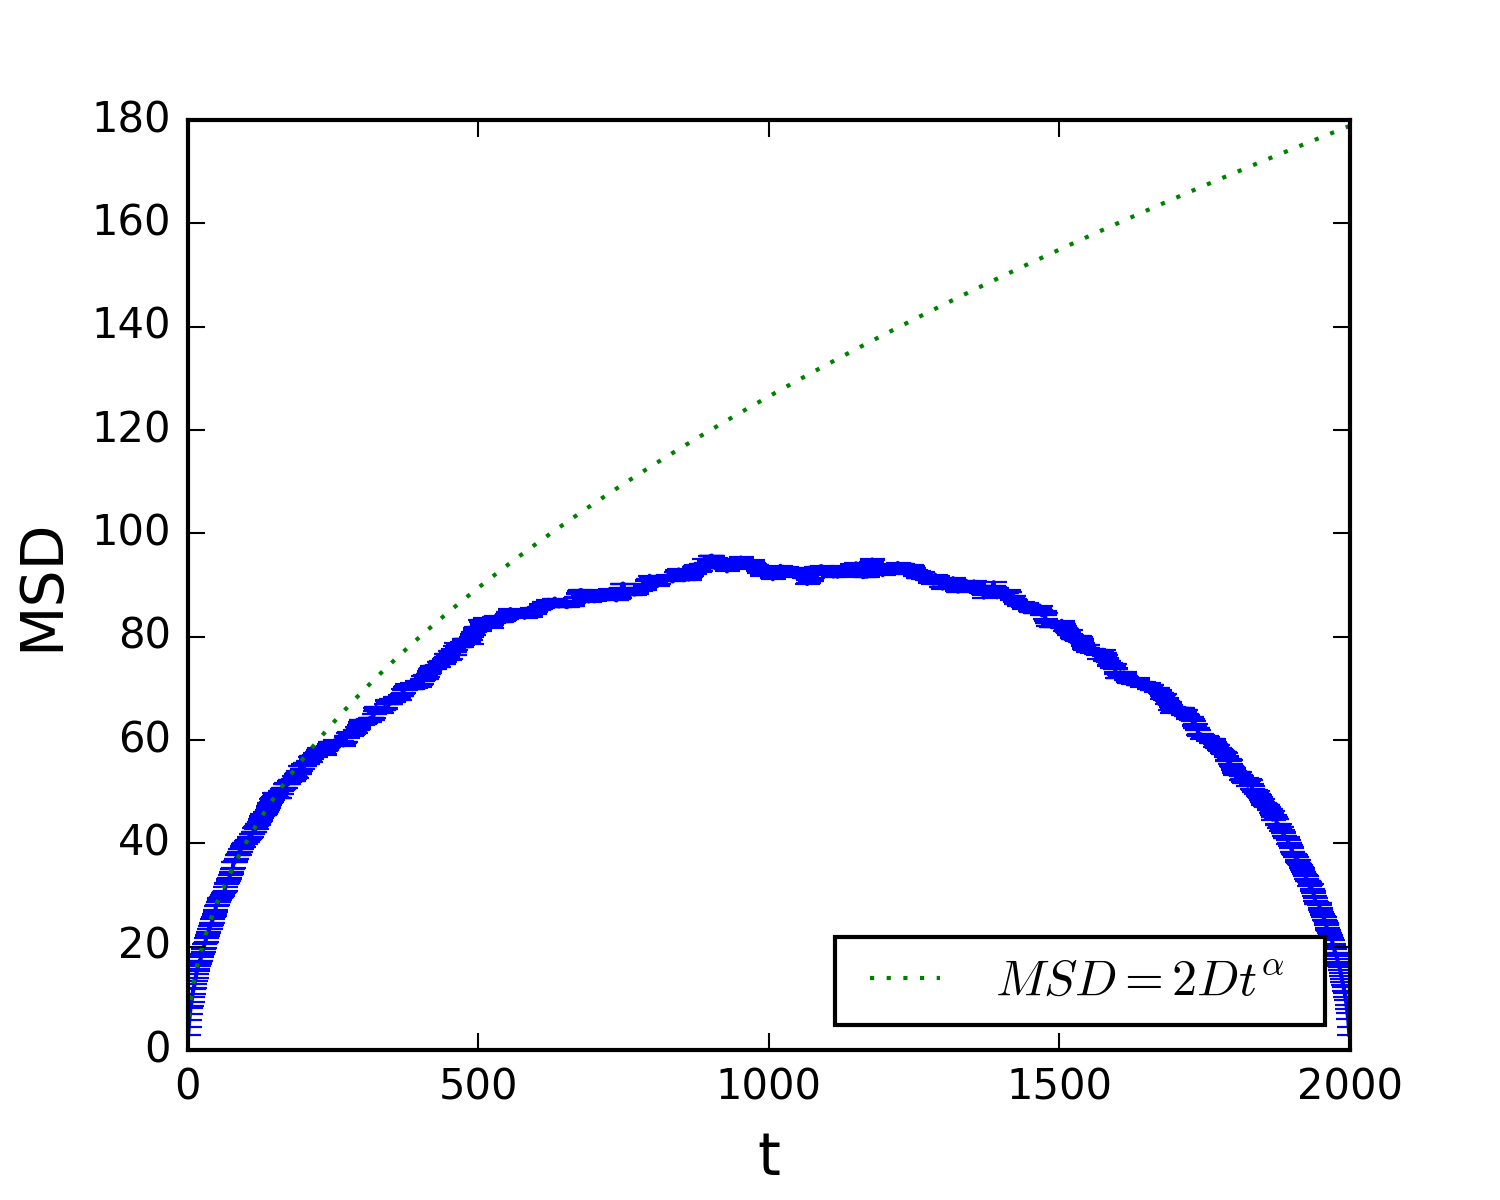
\includegraphics[width=\linewidth]{./data/nocorrectionmsd.png}
  \captionsetup{width=0.9\linewidth}
  \captionof{figure}{Ensemble MSD without the correction introduced in \cref{correction}  }
  \label{fig:6}
\end{minipage}%
\begin{minipage}{.5\textwidth}
  \centering
  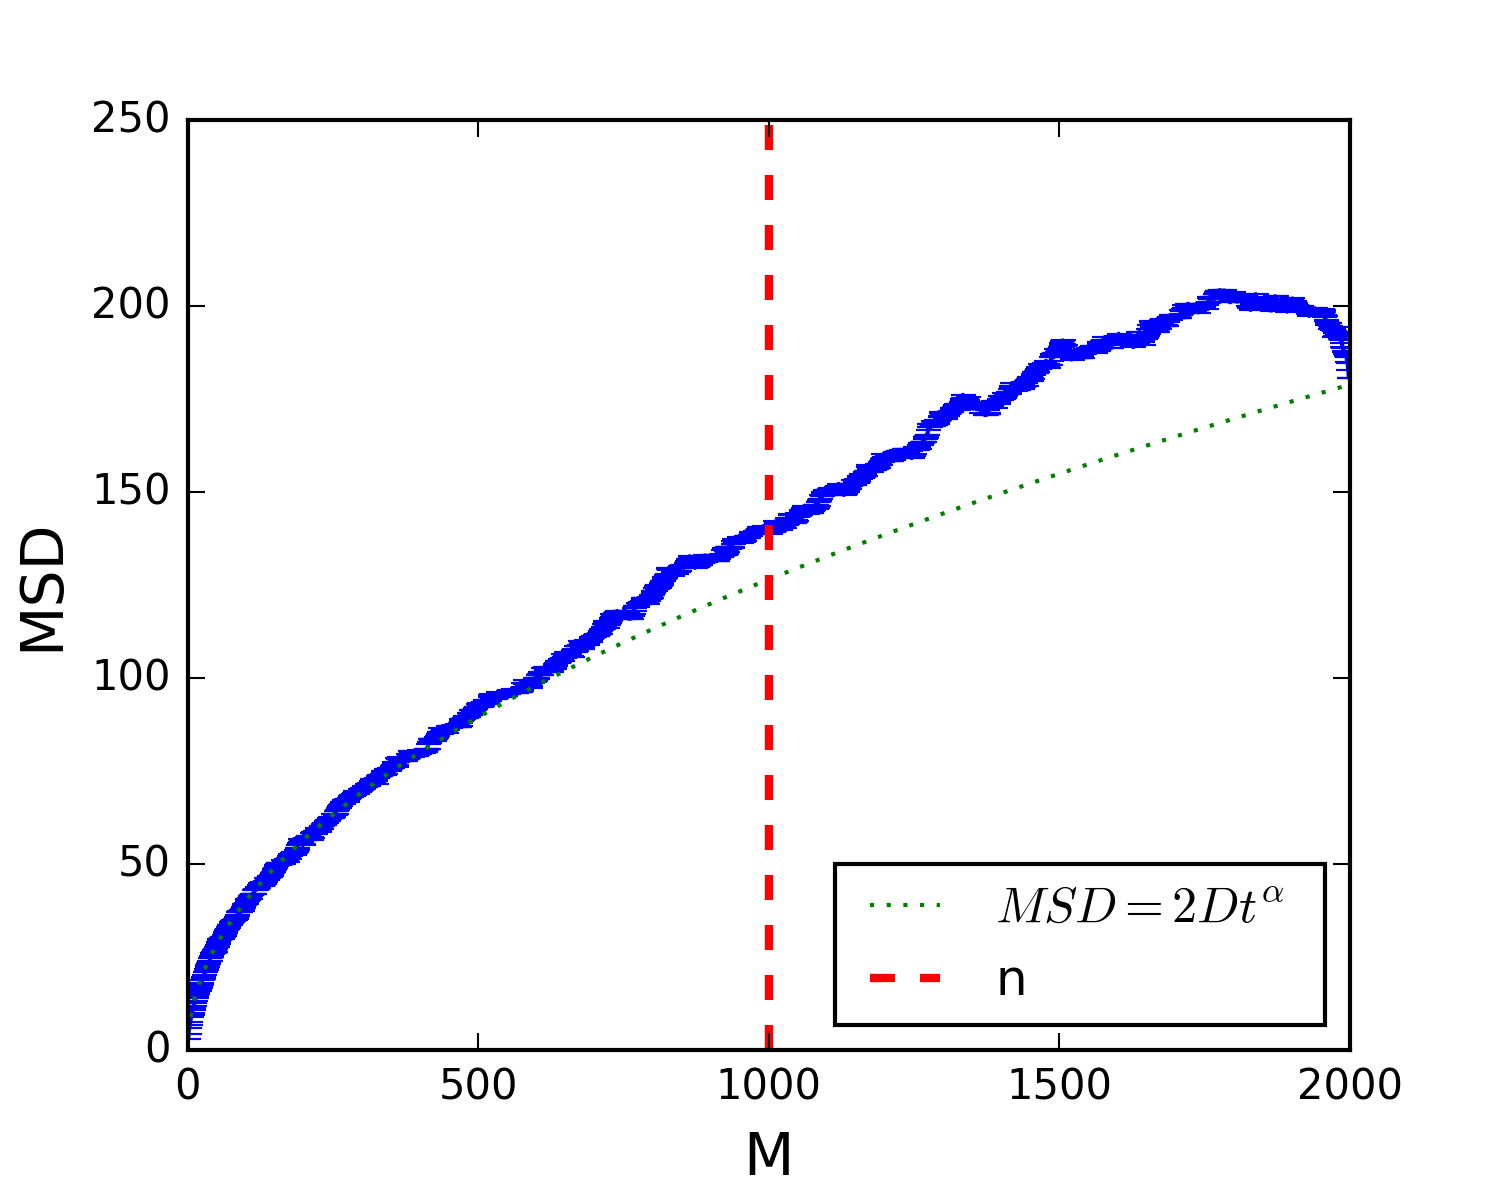
\includegraphics[width=\linewidth]{./data/withcorrection_nocutoff.png}
  \captionsetup{width=0.9\linewidth}
  \captionof{figure}{Ensemble MSD with correction introduced in \cref{correction}. The side of the red bar indicates the remaining increments for $M=2n$ }
  \label{fig:5}
\end{minipage}
\end{figure}
 This equation would be correct if we assumed fractional Brownian motion to be a Markovian process which certainly is not the cause. This is also the reason why k have been chosen to be $2n$. The presumption is, that the impact of the approximation would be negligible with increasing distance to $\Delta R_{2n}$ and negligible at $\Delta R_{n}$.  
 %\item Laut dem Davies Harte Algorithmus wird außerdem das n-te Inkrement im Frequenzraum %umgeändert:
 %\begin{align}
 %\eta_{fbr_{g=n}} =\sqrt{Re(Z_g 2 n)} \mathcal{N}(0,1) 
 %\end{align}
 % Noch nicht verstanden warum!!
 \item With the reverse Fourier transform the fractional Brownian noise increments in the time domain result in:
 \begin{align}
 \xi_{k}= \frac{1}{2n} \sum_{l=0}^{2n-1}  \tilde{\xi}_l e^{\frac{2 \pi i l k }{2n}} \Delta z
 \end{align}
Only the first half of the increments are taken  into account $\xi_{j}$ für $j=(0,1,..,n)$.
\end{enumerate}
The described algorithm can be performed for every Cartesian component of the three dimensional fractional Brownian motion. The Cartesian component are not correlated.
\subsubsection{Analyse of Algorythm}


\begin{figure}[h]
\centering
\begin{minipage}{.5\textwidth}
  \centering
  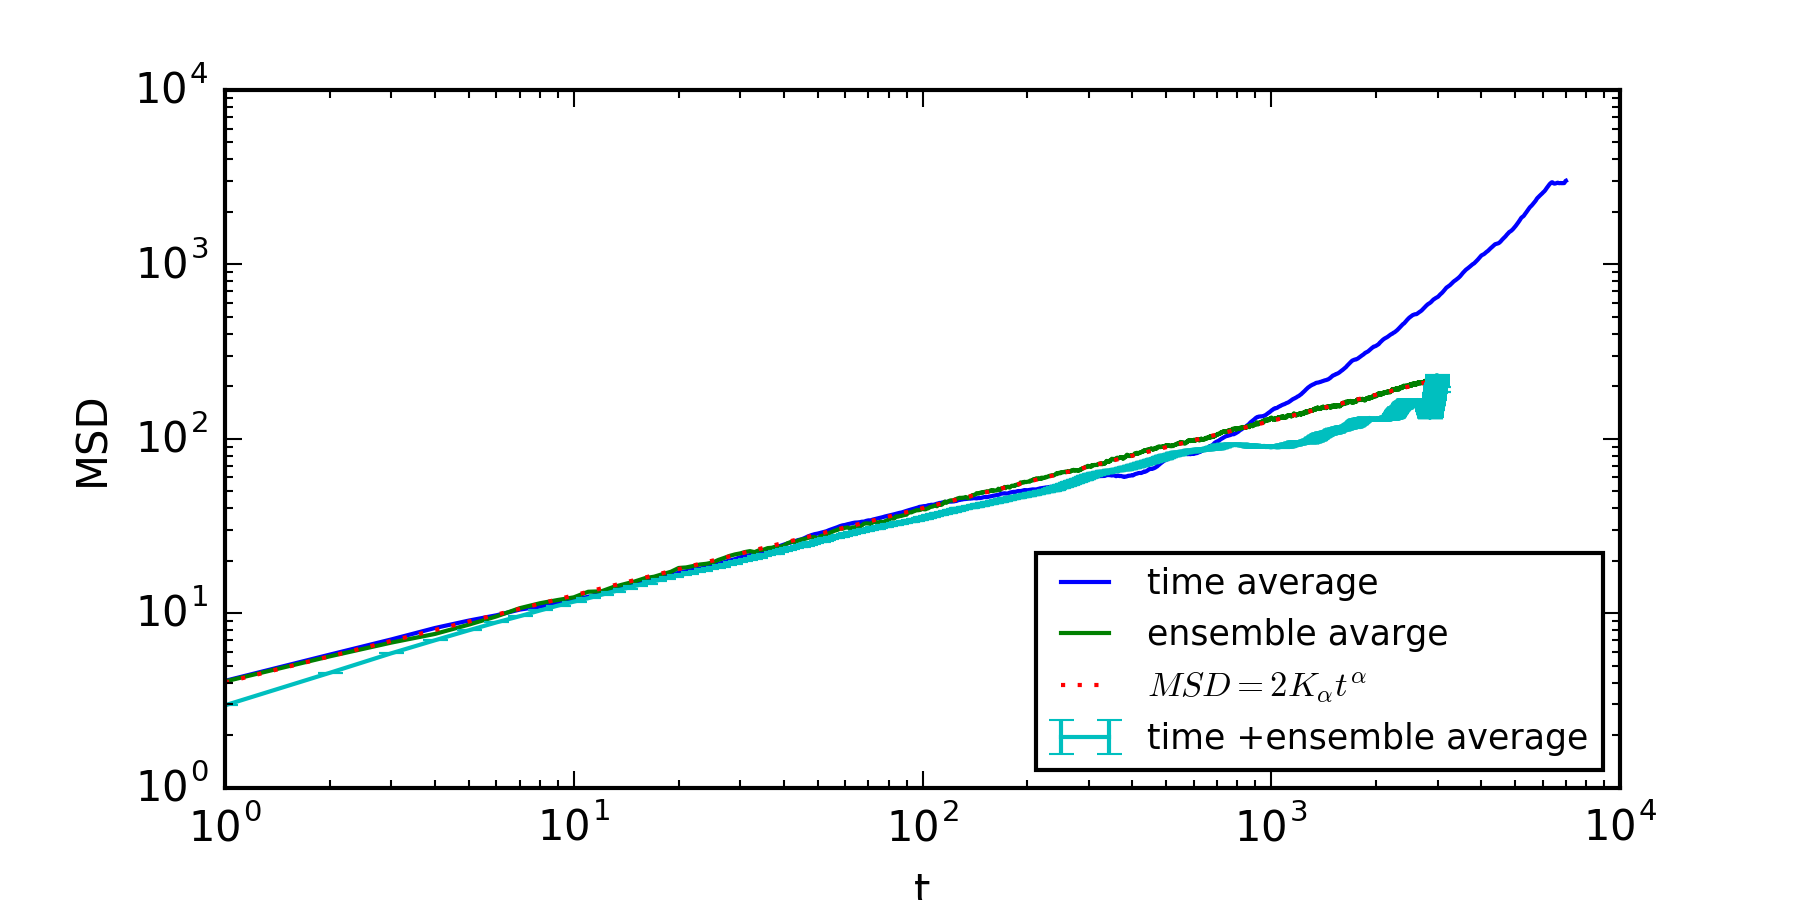
\includegraphics[width=\linewidth]{./data/averages_comparison.png}
  \captionsetup{width=0.9\linewidth}
  \captionof{figure}{Comparison of Mean-Square-Displacements between time-average, ensemble-average and time-ensemble-average(for $D=2$, $\alpha=0.5$, $\Delta t=1$). }
  \label{fig:4}
\end{minipage}%
\begin{minipage}{.5\textwidth}
  \centering
  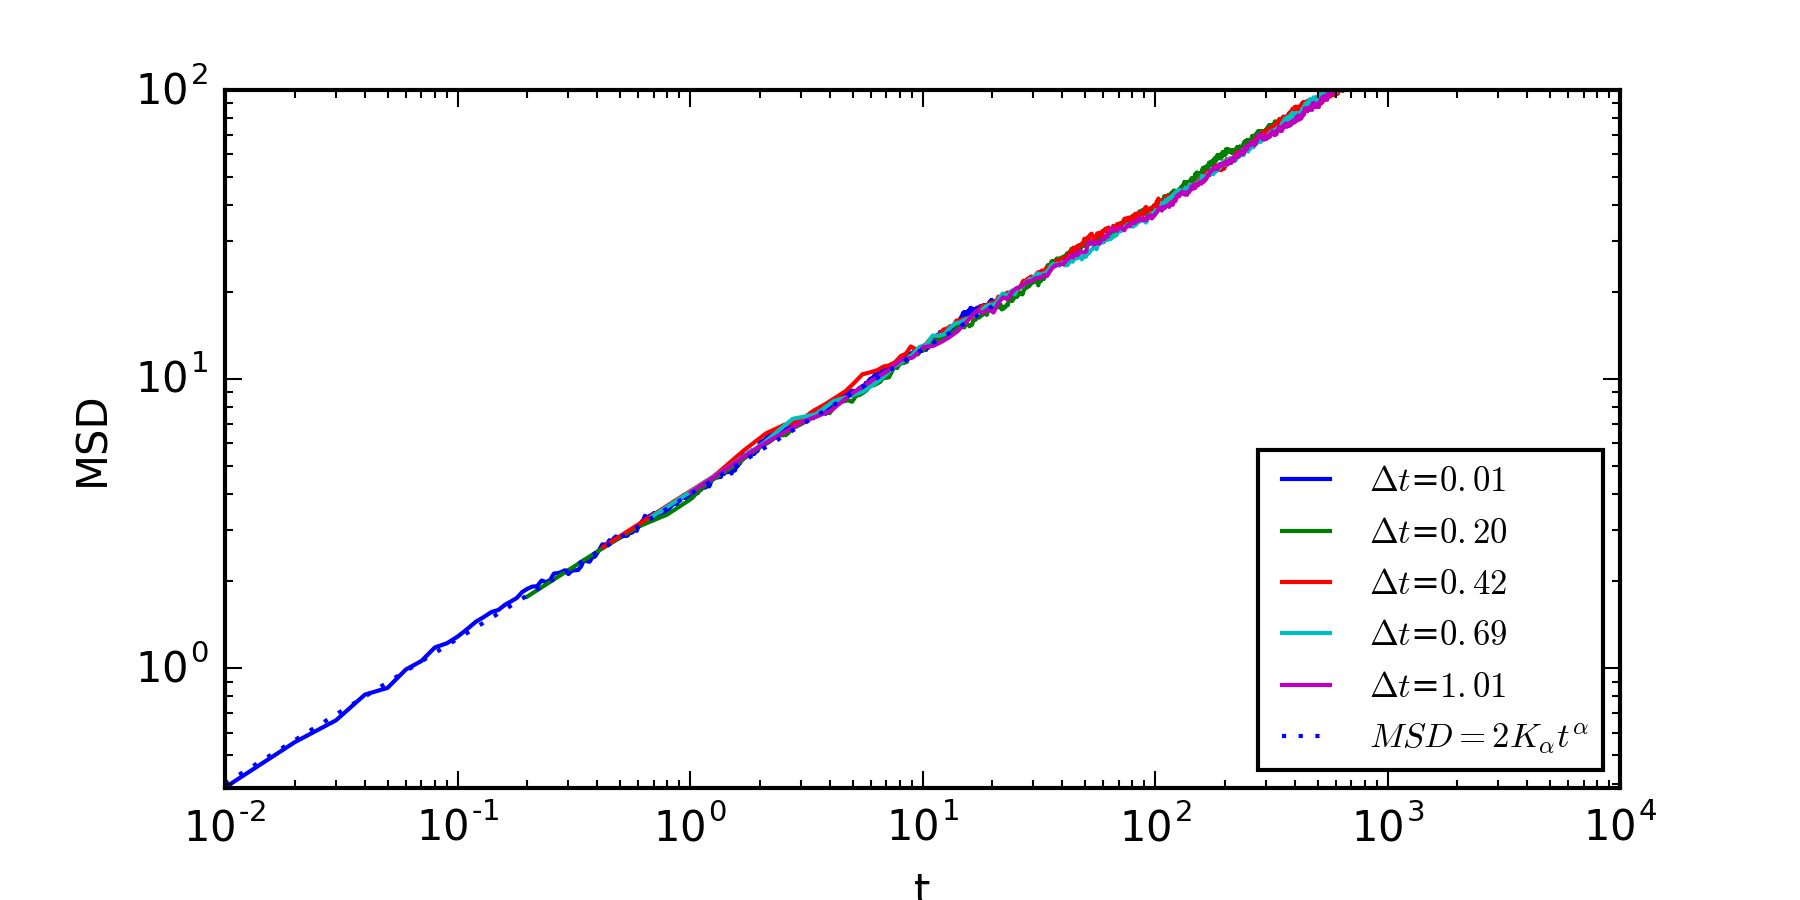
\includegraphics[width=\linewidth]{./data/dt_change.png}
  \captionsetup{width=0.9\linewidth}
  \captionof{figure}{Comparison of ensemble averaged Mean-Square-Displacements with different $\Delta t$(for $D=2$, $\alpha=0.5$). }
  \label{fig:3}
\end{minipage}
\end{figure}


\begin{figure}[h]
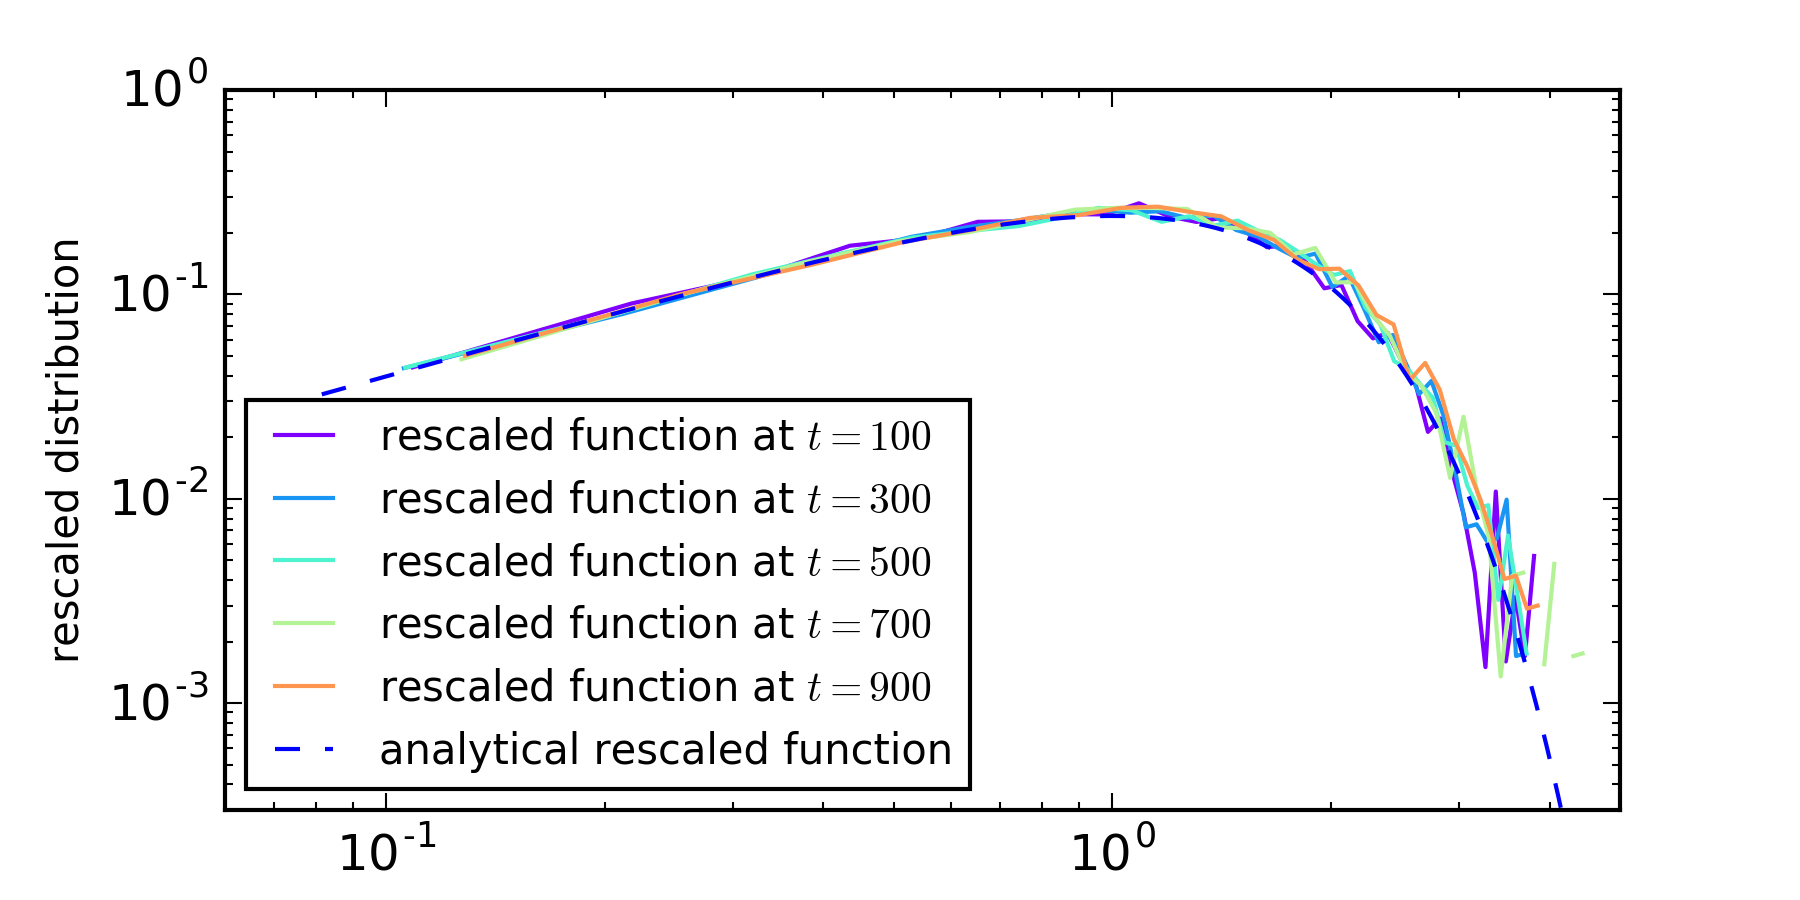
\includegraphics[width=\textwidth]{./data/rescaled.png}
\caption{rescaled functions}
 \centering
\end{figure}

\begin{figure}[h]
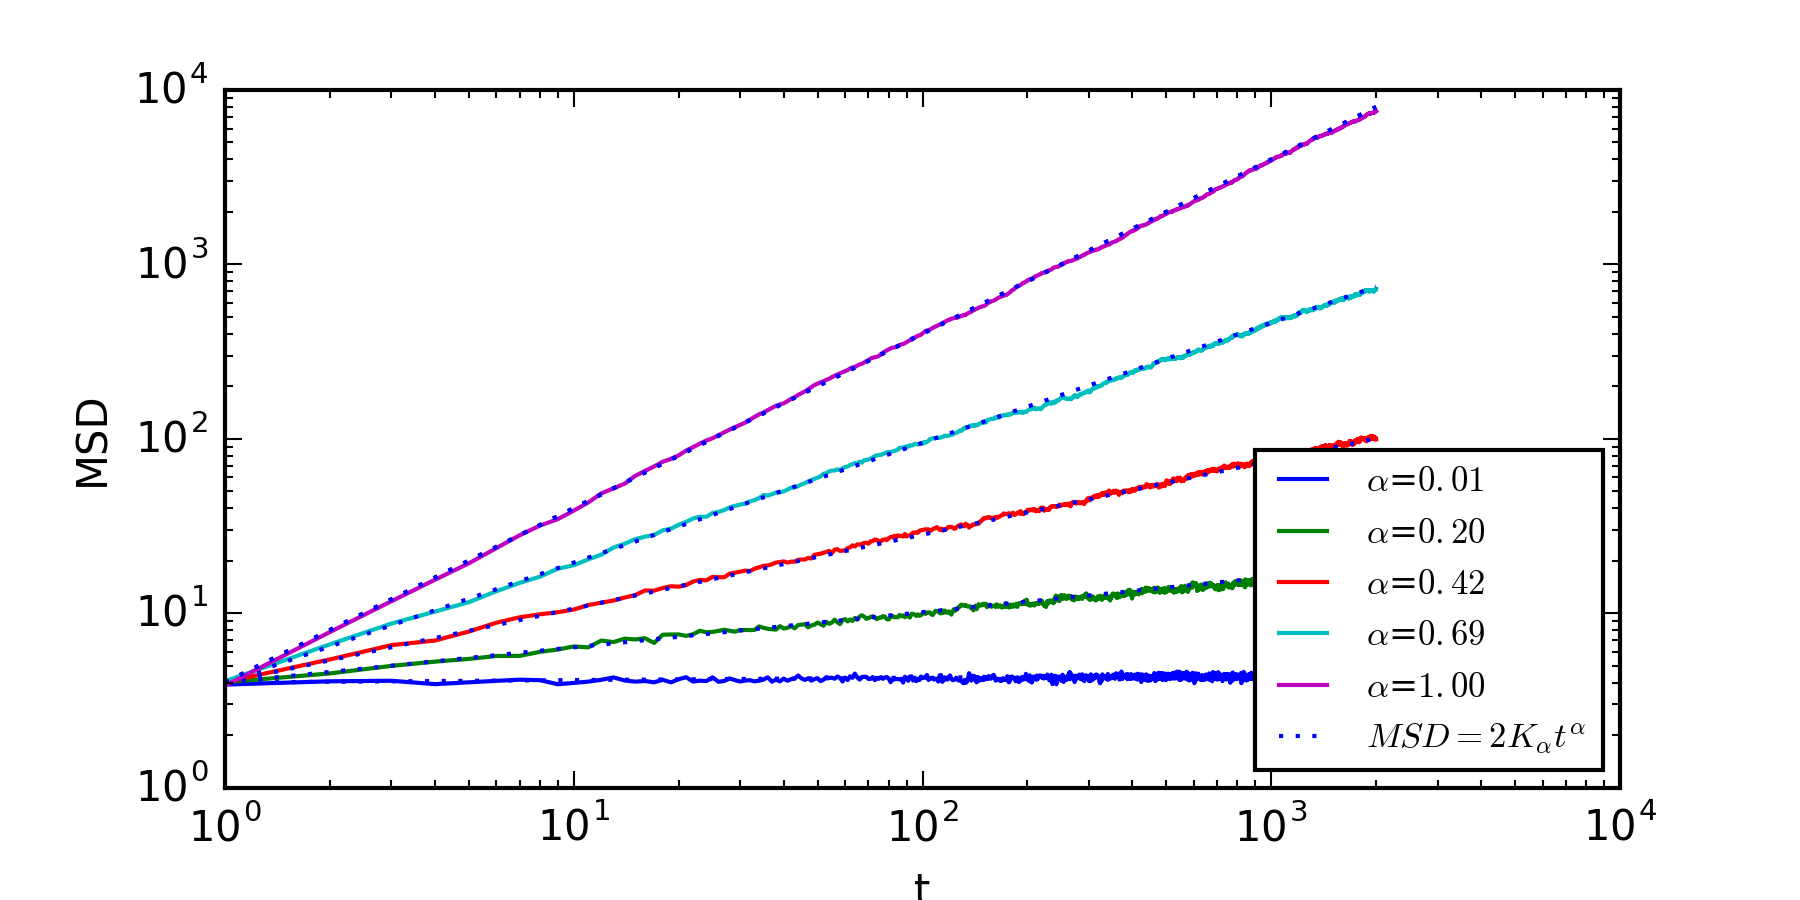
\includegraphics[width=\textwidth]{./data/alpha_change.png}
\caption{Mean-Square-Displacement for different $\alpha$. With $K_{\alpha}=2$ , $N=2000$, $n=2000$ , $\Delta t = 1$, $M=2n$ }
 \centering
\end{figure}

\begin{figure}[h]
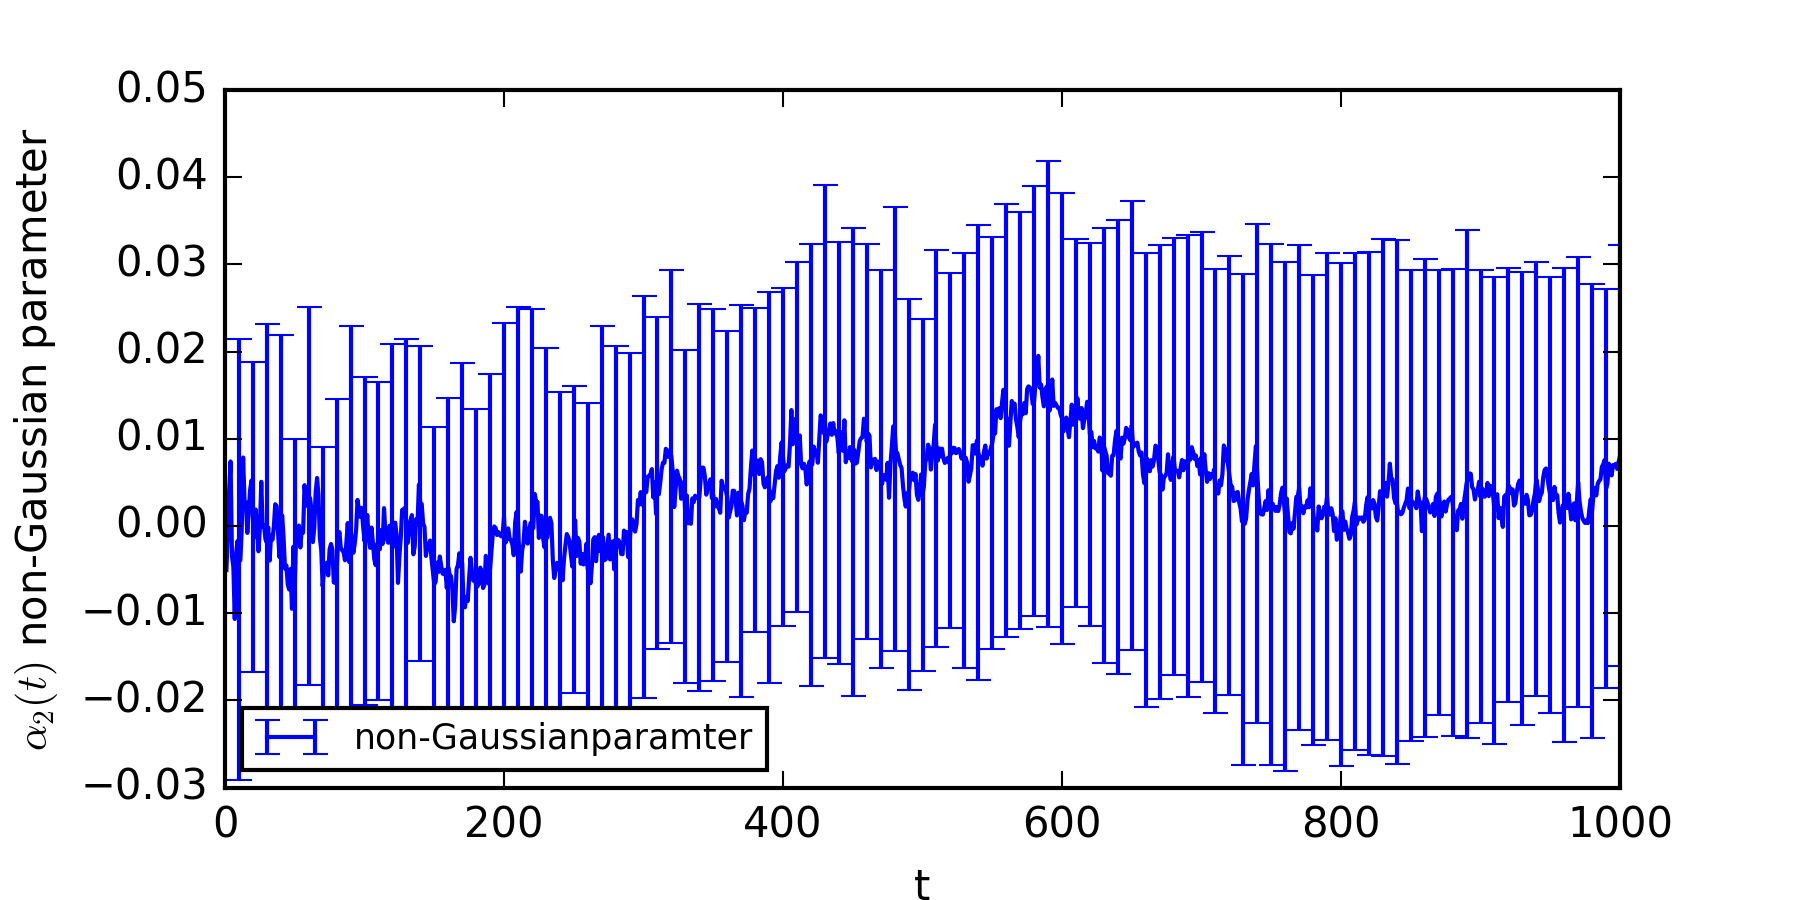
\includegraphics[width=\textwidth]{./data/nongaussian.png}
\caption{Non-Gaussian-Parameter With $K_{\alpha}=2$ , $N=5000$, $n=1001$ , $\delta t = 1$, $M=2n$ averaged over $30$ non-Gaussian-Parameter with its variance displayed as an error bar.}
 \centering
\end{figure}


\begin{figure}[h]
\centering
\begin{minipage}{.5\textwidth}
  \centering
  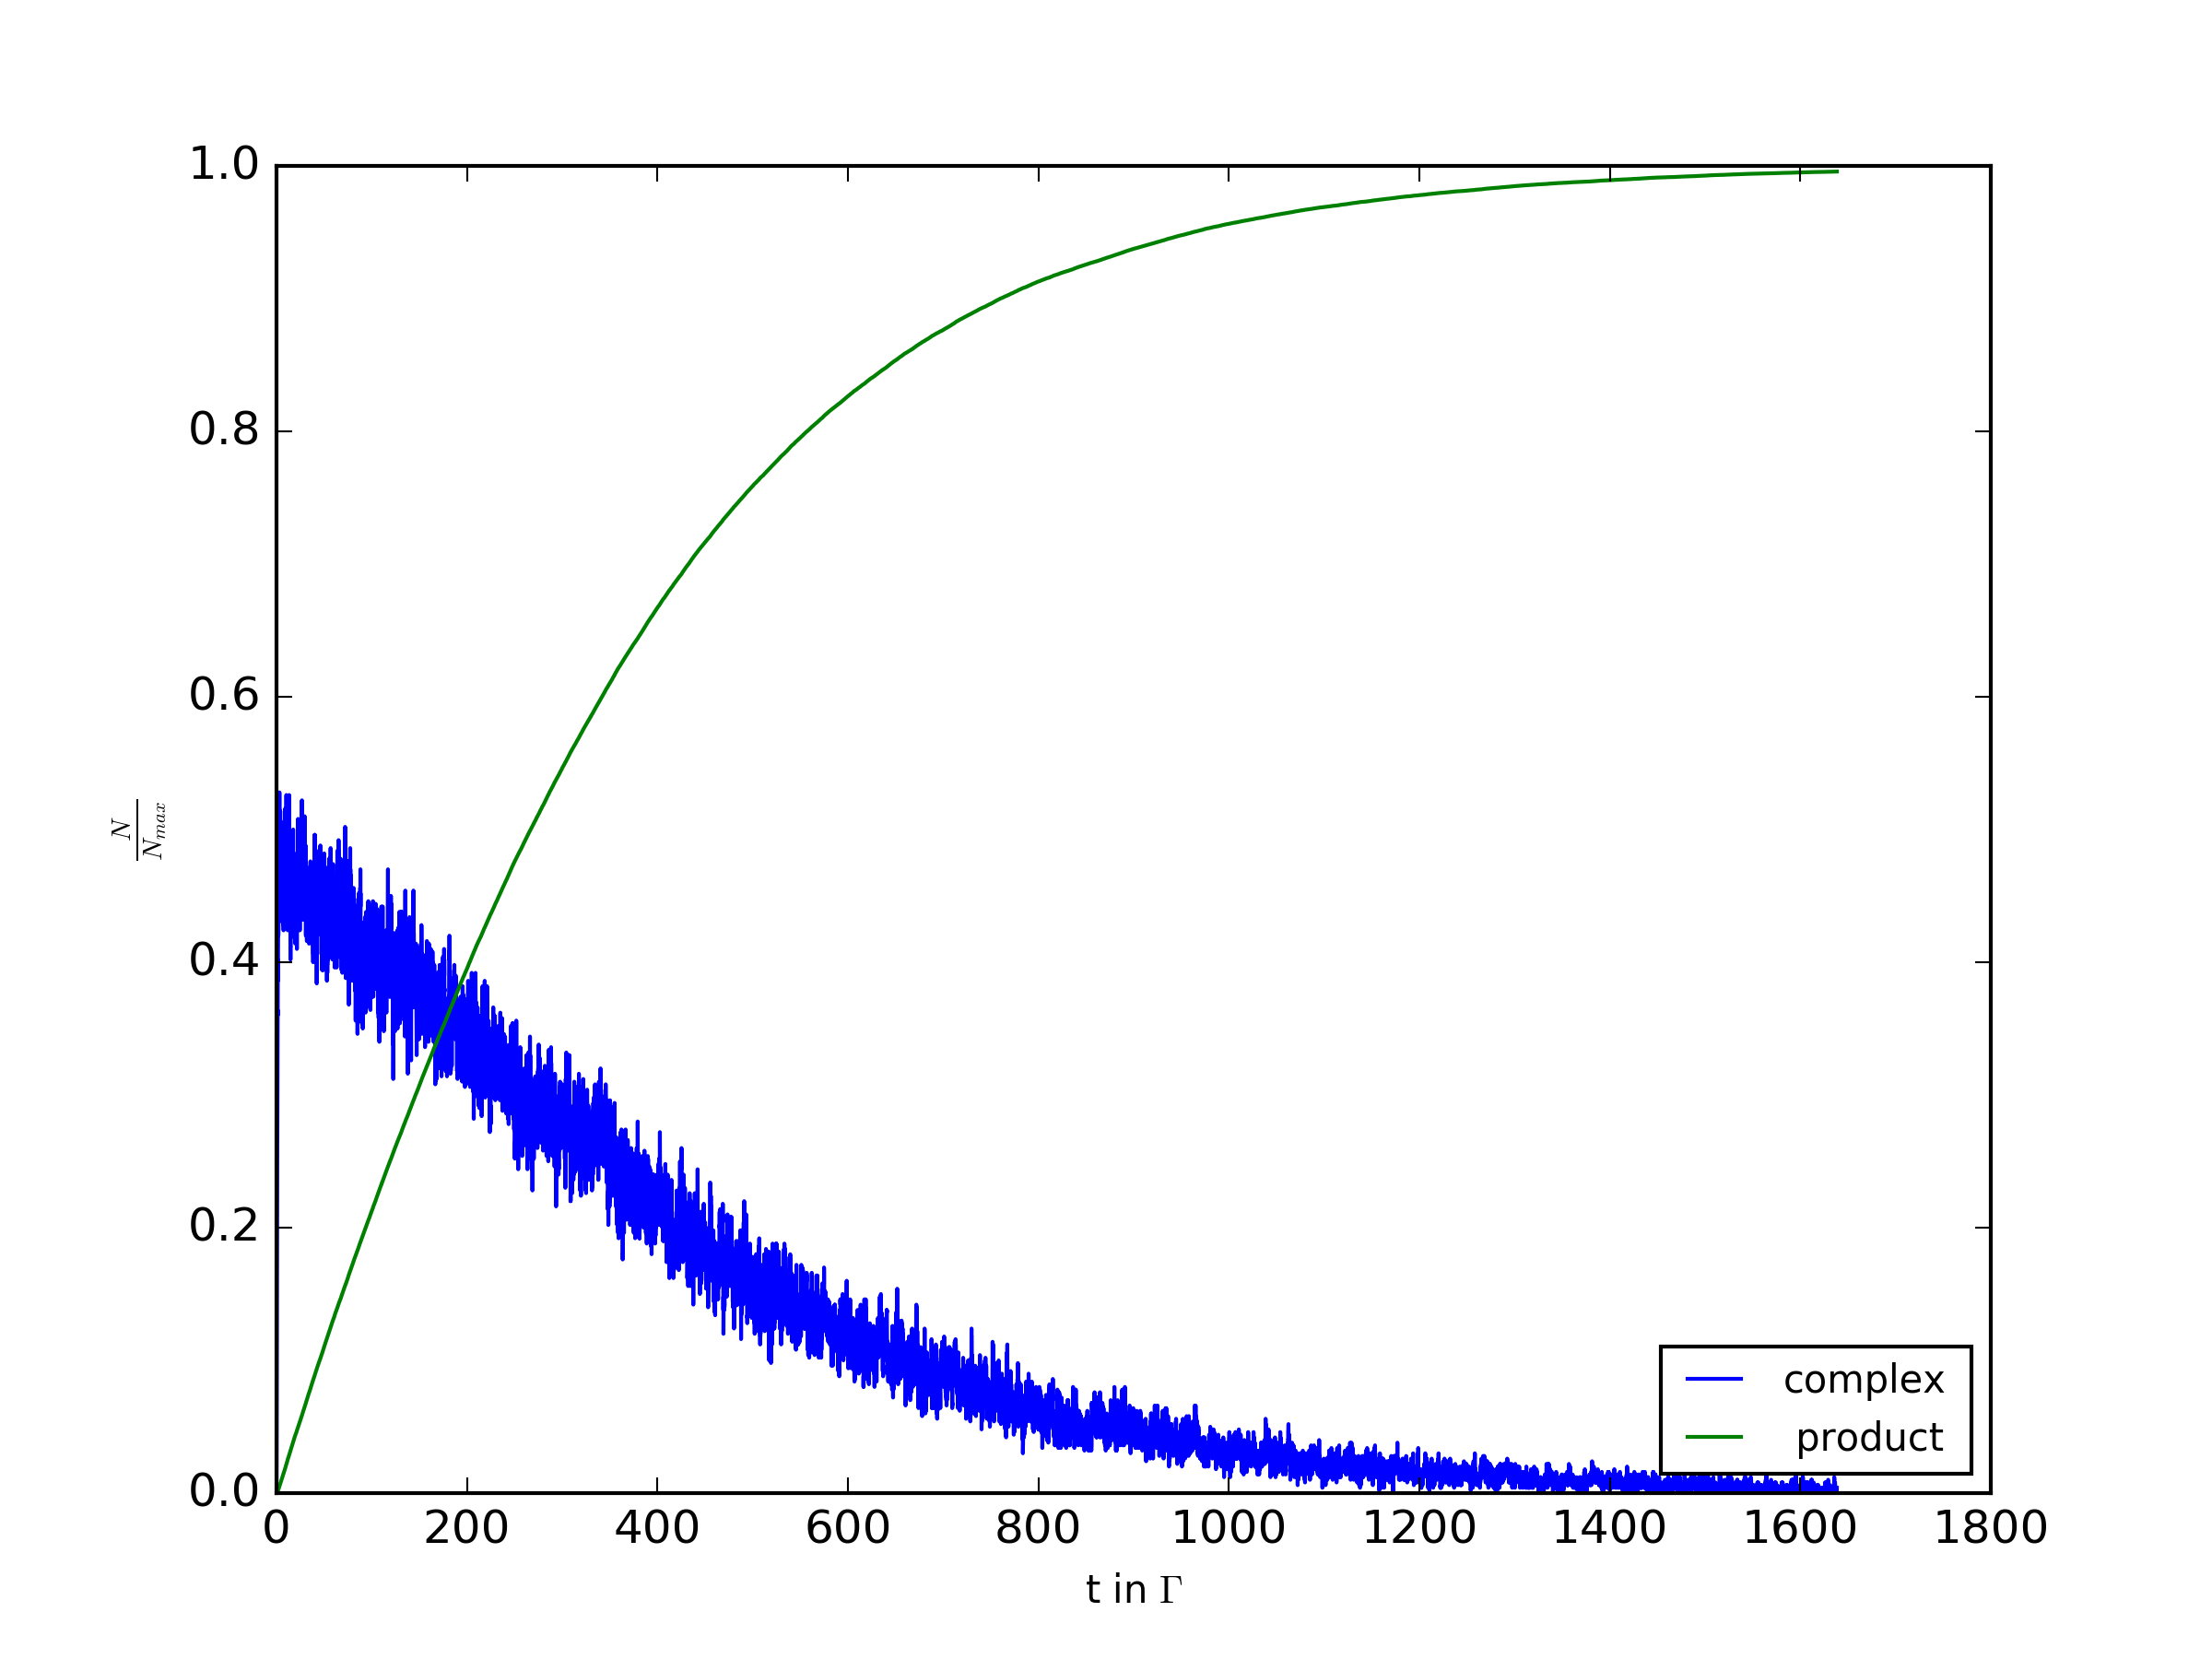
\includegraphics[width=\linewidth]{./data/profiling_length.png}
  \captionsetup{width=0.9\linewidth}
  \captionof{figure}{Profiling c++ and python code in respect to trajectory length $n$}
  \label{fig:1}
\end{minipage}%
\begin{minipage}{.5\textwidth}
  \centering
  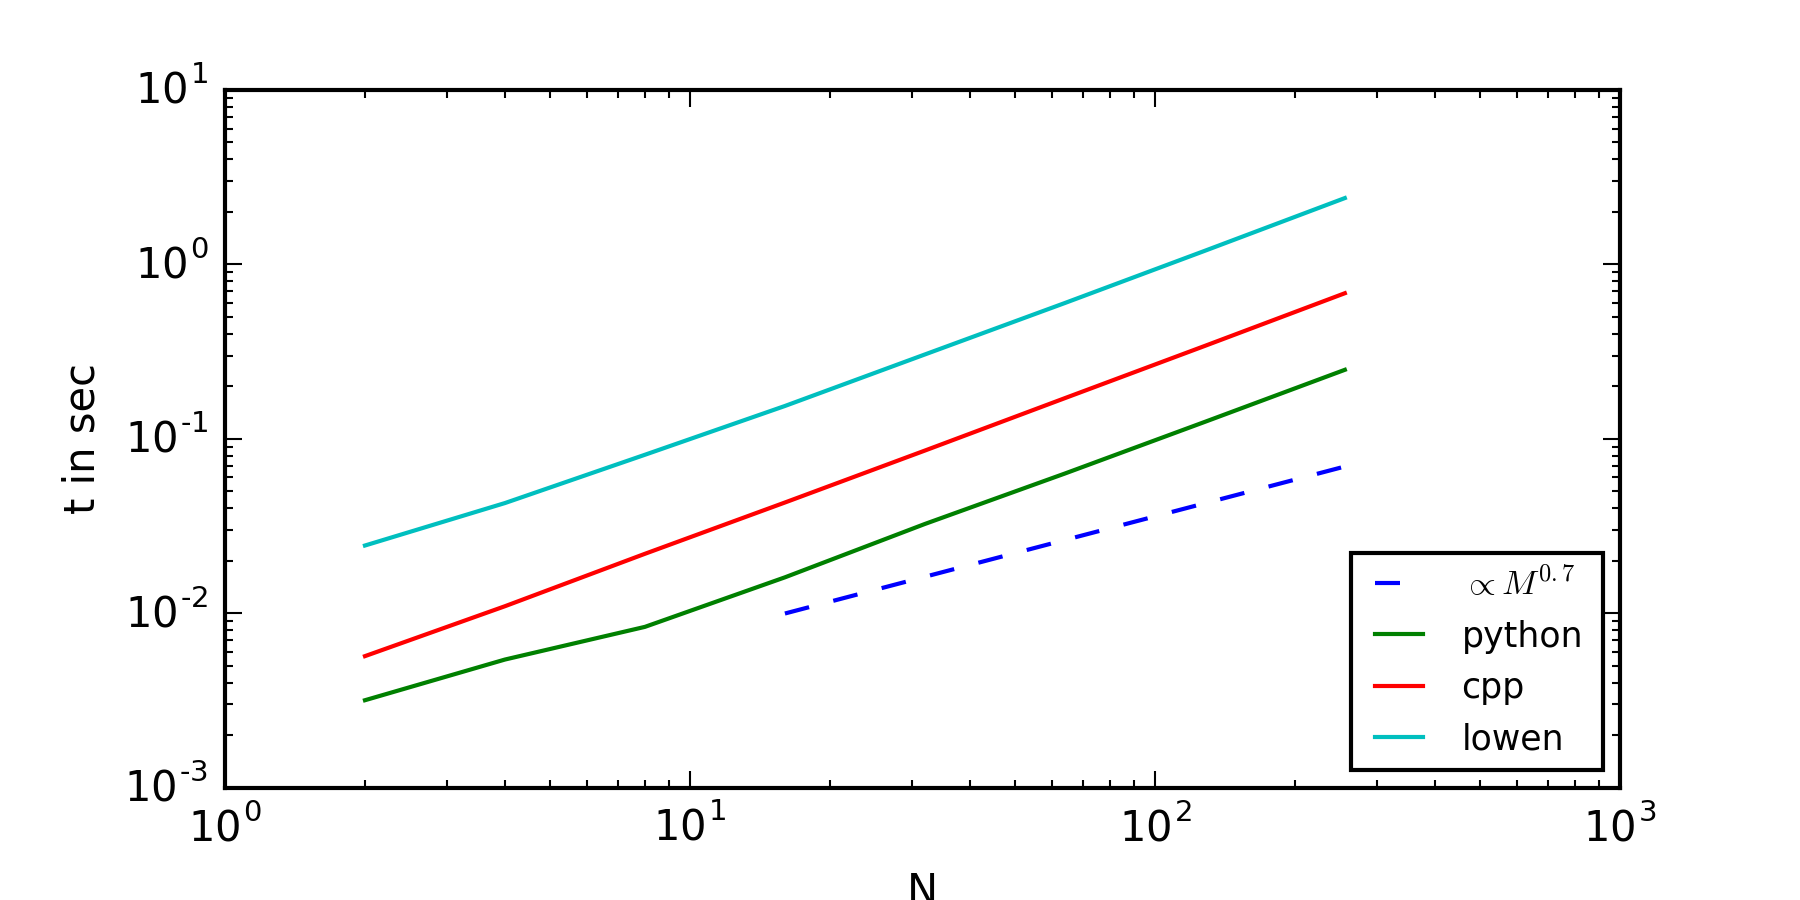
\includegraphics[width=\linewidth]{./data/profiling_particle.png}
  \captionsetup{width=0.9\linewidth}
  \captionof{figure}{Profiling c++ and python code in respect to trajectory number $N$}
  \label{fig:2}
\end{minipage}
\end{figure}



\chapter{Reactions-Diffusion-Dynamics}

Start with Fick's law \cref{eq:ficks} and continuity equation than Smoluchowski equation, reaction coefficient in diffusion controlled reactions.
 but also to provide a Fractional Brownian Motion Integrator implemented into a \textbf{Rea}ction \textbf{D}iffusion \textbf{Dy}namics software (ReaDDy). ReaDDy being a particle-based \textbf{Rea}ction \textbf{D}iffusion \textbf{Dy}namics software is acting on a macromolecular level. (cite readdy paper)
 
 check book zwanzig non-equilibrium stat. mech.
 
\chapter{Status Quo \& Outlook}
\chapter{Appendix}
\section{From Central Limit Theorem to Gaussian Distribution}\label{append:CLT}
In the following the Central Limit Theorem will be applied to calculated the distribution of Y,  $\rho(y)dy=P(y<Y<y+dy)$ in the limit of large N , with Y being defined as the sum of an random variable:
 \begin{align}
  Y = \frac{1}{\sqrt{N}} \sum_{j=1}^N X_j \label{eq:CLT1}
 \end{align}
The Generating function for a random variable $Y$ is: 
\begin{align}
 G_Y(k)=\langle e^{ikY}\rangle = \int e^{ikY} \rho(y)dy
\end{align}
\cref{eq:CLT1} can be inserted into the generating function, which results in:
\begin{align*}
G_Y(k)=\langle e^{\frac{ik}{\sqrt{N}} \sum_{j=1}^N X_j}\rangle \\
G_Y(k)=\langle \prod_{j=i}^N e^{\frac{ik}{\sqrt{N}} X_j} \rangle 
\end{align*}
If all $X_j$ are independent, then:
\begin{align}
 G_Y(k)= \prod_{j=i}^N \langle e^{\frac{ik}{\sqrt{N}} X_j} \rangle =e^{\sum_{j=1}^N A_j (\frac{k}{\sqrt{N}})} \\ \nonumber \text{ with } A_j(\frac{k}{\sqrt{N}})= ln \langle e^{\frac{ik}{\sqrt{N}} X_j} \rangle 
\end{align}
For large N behaviour, we assume $\frac{k}{\sqrt{N}} << 1$ and expand
\begin{align}
 A_j(\frac{k}{\sqrt{N}}) = ln(1+ \langle X_j \rangle \frac{ik}{\sqrt{N}} - \langle X_{j}^2 \rangle \frac{k^2}{2N}+\mathcal{O}(N^{- \frac{3}{2}}))
\end{align}
 with a finite variance $ \sigma_i^2=\langle X_{i}^2\rangle $ and the mean $\langle X_{i}\rangle = 0$
\begin{align}
 A_j(\frac{k}{\sqrt{N}}) = -\sigma_j^2 \frac{k^2}{2N}+\mathcal{O}(N^{- \frac{3}{2}}))
\end{align}

Thus, the generating function for large N is:

\begin{align}
 G_Y(k)=e^{- \frac{\sigma^2 k^2}{2}} \\ \nonumber
 \text{ with } \sigma =  \frac{1}{N} \sum_{j=1}^N \sigma_j^2 
\end{align}
The distribution of Y can be calculated via the inverse Fourier Transform:
\begin{align}
 \rho(y) &=\frac{1}{2 \pi} \int_{-\infty}^{\infty} e^{- \frac{\sigma^2 k^2}{2}} e^{i k y} dk \\  
 &=\frac{1}{\sqrt{2 \pi} \sigma } e^{-\frac{y^2}{2 \sigma^2}}
\end{align}
$\rho(y)$ results in a Gaussian distribution.

\section{From Gaussian Propagator to Gaussian distribution}\label{baystheorem}
The conditional distribution function to be in $x$ at time $t$ if visited position $y$ at time $s$   can be written due to Bayes' theorem as a transition probability from $y$ to $x$ in time $t-s$ multiplied with the probability to be in $y$ at time $s$:
\begin{align}
 \rho_{t,s}(x,y)=T_{t-s}(x|y) \rho_s(y)
\end{align}
Further due to particle conservation another relation holds:
\begin{align}
 \rho_{t}(x)= \int \rho_{t,s}(x,y) dy
\end{align}
Having an initial condition $\rho_{s}(x)= \delta(x-y)$:
\begin{align}
 \rho_{t,s}(x|y)&= \int \rho_{t,s}(x,y) dy = \int T_{t-s}(x|y) \rho_s(y) dy\\
 &= \int T_{t-s}(x|y) \delta(x-y) dy 
 = T_{t-s}(x|y)
\end{align}
\section{Einstein Formula} \label{einsteinrealtionappendix}
The derivative of the mean variance of the Gaussian distribution in respect to time is defined as:
\begin{align}
 \frac{d}{dt}  \delta \bm{r}^2(t)&=\frac{d}{dt} \langle \Delta \bm{ R}^2(t)\rangle  =\frac{d}{dt} \int d\bm{r} \bm{r}^2 c(\bm{r},t)=\int d\bm{r} \bm{r}^2 \frac{\partial}{\partial t} c(\bm{r},t) 
\end{align}
Fick's second law can be applied:
\begin{align}
&= D \int_{-\infty}^{\infty}d\bm{r} \bm{r}^2 \Delta c(\bm{r},t)  
\end{align}
Assuming a reasonable assumption  $c(\pm \infty,t)=0$  and two times partial integration one can derive:
\begin{align}
&= \left[ \right]_{-\infty}^{\infty}-2 D \int_{-\infty}^{\infty} d\bm{r} \bm{r} \nabla c(\bm{r},t) \\ &= 2 D d \int_{-\infty}^{\infty} d\bm{r} c(\bm{r},t) =2dD
\end{align}
In previous equations partial integration  By integration the initial condition $\bm{r}(0) = 0$,  one gets the Einstein Formula: $\langle (\bm{r}(t)-\bm{r}(0))^2)\rangle= 2dDt$

check book zwanzig

\section{Autocorrelation Function for fBm}
Subsequently, the VACF in the frequency domain for Fractional Brownian motion can be calculated. The MSD is $\delta r^{2}(t)= < \Delta R(t)>=2dK_{\alpha}t^{\alpha}$ with $K_{\alpha}$ being the generalized diffusion-coefficient:
\begin{align*}
 \tilde{Z}(z)&=\int_{0}^{\infty} d t e^{izt} Z(t) \\
 &=2 d \int_{0}^{\infty} d t e^{izt} \left[\frac{d^2}{dt^2}\delta r^2 (t) \right]
\end{align*}
\begin{align*}
  \stackrel{par. integ.}{=} 2d \left( \underbrace{\left [ e^{izt}\overbrace{ \frac{d^2}{dt^2} 2dK_{\alpha}t^{\alpha}}^{=A(t)} \right]_{0}^{\infty}}_{\stackrel{\alpha < 2} {=} 0}-\int_{0}^{\infty} d t e^{izt} \left[\frac{d}{dt}\delta r^2 (t)\right] \right) 
 \end{align*}
 \begin{align*}
 A(t)=\frac{d}{dt}\overbrace{ \left [\frac{2d K_{\alpha}t^{\alpha-1}}{\alpha} \right ]}^{B(t)}=\frac{2d K_{\alpha}t^{\alpha-2}}{\alpha+(\alpha-1)}
\end{align*}

\begin{align*}
 \tilde{Z}(z) & \stackrel{par. integ.}{=} - 2d \left( \underbrace{\left [ e^{izt}\overbrace{ \frac{d}{dt} 2dK_{\alpha}t^{\alpha}}^{=B(t)} \right]_{0}^{\infty}}_{\stackrel{\alpha < 1} {=} 0}-\int_{0}^{\infty} d t e^{izt} \delta r^2 (t) \right) \\
  & = \int_{0}^{\infty} d t e^{izt} \delta r^2 (t)  \stackrel{\operatorname{Im}(z)> 0} {=}  K_{\alpha} \Gamma(1+\alpha)(i z)^{1-\alpha}
\end{align*}
%\subsection{Code:Gebrochen-rationale Brownische Bewegung}
%\lstinputlisting[language=Python]{../simulation.py}

\nocite{}

%\printindex
\bibliography{literatur}
\bibliographystyle{plain}

\end{document}